% !TeX encoding = utf8
% !TeX program = xelatex
% !BIB program = bibtex
% -*- coding:utf-8 mod:LaTeX -*-

% Paper 3: Open-Set SC-BSS
% Template: elsarticle (review format) — target venue: Physical Communication (Elsevier)

\documentclass[review,12pt]{elsarticle}

\usepackage{graphicx}
\usepackage{booktabs}
\usepackage{amsmath,amssymb}
\usepackage{url}
\usepackage{xcolor}
\usepackage[mode=text]{siunitx}
\sisetup{locale=US}

\usepackage{hyperref}
\hypersetup{hidelinks,
  colorlinks=true,
  allcolors=black,
  pdfstartview=Fit,
  breaklinks=true}

\usepackage{lineno}
\modulolinenumbers[5]

\usepackage{float}

\emergencystretch=1.5em

\newcommand{\snr}{\mathrm{SNR}}

\journal{Physical Communication}

\begin{document}

\begin{frontmatter}

\title{Open-Set Single-Channel Blind Source Separation:\\Per-Source Modulation Detection is SNR-Dependent}

\author[1]{Bin Nong\corref{cor1}}
\ead{nongbin@tfswufe.edu.cn}
\author[2]{Weihong Fu}
\author[3]{Zhuoyun Jiang}

\affiliation[1]{organization={Tianfu College of Southwestern University of Finance and Economics}, city={Mianyang}, state={Sichuan}, postcode={621000}, country={China}}
\affiliation[2]{organization={School of Telecommunications Engineering, Xidian University}, city={Xi'an}, state={Shaanxi}, postcode={710071}, country={China}}
\affiliation[3]{organization={School of Health Science and Engineering, University of Shanghai for Science and Technology}, city={Shanghai}, postcode={200093}, country={China}}

\cortext[cor1]{Corresponding author.}

% ======================================================================
\begin{abstract}
Existing single-channel blind source separation (SC-BSS) systems for
co-frequency communication signals assume that the modulation format of
every source is known a priori; a practical receiver has no such
guarantee. We reframe SC-BSS as an \emph{open-set recognition problem}:
joint separation and per-source modulation identification with rejection
of unseen modulations. On a new open-set SC-BSS benchmark (four known /
four held-out modulations, three evaluation protocols), we show that
standard out-of-distribution (OOD) scorers (six post-hoc methods from
the Energy/MSP/ODIN and Prototype/VOS/Mahalanobis families) over
per-source embeddings from a lightweight complex-valued backbone
($\sim$69K parameters) are \emph{at chance when pooled across
SNR---but strongly complementary when conditioned on SNR}: Prototype/VOS
reach 0.84 AUROC at \SI{10}{dB} yet collapse below \SI{0}{dB}, where the
Energy score instead peaks at 0.74. Exploiting this structure, a
training-free \emph{SNR-routed ensemble} lifts the weighted-average AUROC
from 0.526 (best single scorer) to 0.625, and degrades gracefully
($\geq 0.576$) under up to \SI{6}{dB} of SNR-estimation error. Multi-seed
ablations show the effect is a property of the backbone features, not of
classification-head capacity or of the training loss. To our knowledge
this is the first open-set formulation of SC-BSS, and the first
demonstration that the ranking of per-source OOD scorers inverts with
SNR.
\end{abstract}

\begin{keyword}
Blind source separation \sep Co-frequency communication \sep Open-set
recognition \sep Out-of-distribution detection \sep Modulation
classification \sep Complex-valued neural network
\end{keyword}

\end{frontmatter}

\linenumbers

% ======================================================================
\section{Introduction}
\label{sec:intro}

\emph{Problem and motivation.} Single-channel blind source separation
(SC-BSS) recovers multiple unknown source signals from one observed
mixture~\cite{hou2022single,guo2024single}. For co-frequency
communication signals, existing deep separators assume a closed world:
the modulation format of every source belongs to a known training
alphabet. A deployed receiver (spectrum monitoring, cognitive radio,
electronic warfare) faces transmitters whose waveforms it has never
seen. In such an open environment, a separator that silently treats an
unseen modulation as its nearest known neighbour is not merely
inaccurate---it is confidently wrong, and downstream demodulation fails
without any indication that it has done so. A practical system must
therefore answer two questions jointly: \emph{what are the sources}, and
\emph{do I even know what they are}.

\emph{Gap.} Two literatures meet here and both fall short. The SC-BSS
literature assumes the closed-set prior described above; to our
knowledge no work has asked how a learned separator behaves when one or
both sources carry an unseen modulation. The open-set recognition and
out-of-distribution (OOD) detection
literature~\cite{bendale2016openmax,hendrycks2017msp,liang2018odin,liu2020energy},
on the other hand, evaluates a scorer at a single global operating
point: detection performance is treated as a fixed property of the
model, pooled over whatever test distribution is at hand. Neither side
expects the ranking of OOD scorers to \emph{invert with the operating
SNR}---which
is precisely what we observe in SC-BSS, where the SNR is not merely a
difficulty knob but determines \emph{which} family of OOD scorers works
at all.

\emph{What we do.} We reframe SC-BSS as an open-set recognition problem:
the separator is equipped with a lightweight per-source modulation head
($\sim$8.6K additional parameters), and standard OOD scorers are applied
to the per-source embeddings and logits. Studying the resulting
benchmark across SNR reveals a striking structure that the standard
pooled metric completely hides---and that structure, once seen, admits
an almost embarrassingly simple exploitation: route each sample to the
scorer family known to work at its SNR.

\emph{Contributions.}
\begin{enumerate}
  \item \textbf{Problem and benchmark.} We give, to our knowledge, the
        first open-set formulation of SC-BSS: joint separation with
        per-source modulation identification and rejection of unseen
        modulations, evaluated under kk/ku/uu protocols with 64QAM,
        $\pi$/4-DQPSK, MSK and OFDM-QPSK held out
        (Section~\ref{sec:setup}).
  \item \textbf{Finding.} Per-source OOD detectability is
        \emph{SNR-dependent}: pooled AUROC $\approx 0.50$ masks a strong
        complementary structure (Prototype/VOS effective at
        $\geq\SI{5}{dB}$, Energy at $\leq\SI{0}{dB}$)
        (Section~\ref{sec:trap}).
  \item \textbf{Method.} A training-free \emph{SNR-routed ensemble}
        lifts the weighted-average AUROC from 0.526 (best single scorer)
        to 0.625, within 0.06 of the post-hoc per-SNR oracle, and is
        robust to SNR-estimation error
        (Sections~\ref{sec:routed}--\ref{sec:robust}).
\end{enumerate}

The remainder of the paper is organised as follows.
Section~\ref{sec:related} reviews the literature this work connects. Section~\ref{sec:method} formalises the open-set SC-BSS
problem, describes the backbone and OOD scorers, and introduces the
SNR-routed ensemble. Section~\ref{sec:exp} presents the benchmark
results, the pooled-metric trap, ablations, and robustness analyses.
Section~\ref{sec:disc} discusses why the two scorer families invert
their roles with SNR, and Section~\ref{sec:limit} states limitations.
Section~\ref{sec:concl} concludes.

% ======================================================================
\section{Related Work}
\label{sec:related}

\subsection{SC-BSS for communication signals}

Blind separation of co-frequency communication signals from a single
sensor violates the overdetermined requirement of classical
ICA~\cite{hyvarinen2000ica} and has
driven a line of deep-learning approaches: convolutional separation
networks~\cite{hou2022single}, recurrent
designs~\cite{chen2019deep}, attention-augmented
models~\cite{ma2023novel}, complex-domain
architectures~\cite{guo2024single}, spatial-temporal
fusion~\cite{luo2023single}, and structured state-space
backbones~\cite{s4unet2026}.
Blind separation has also been used as a front-end for co-channel
modulation classification~\cite{deng2024co}, but again under a
closed-set label alphabet.
All of these works evaluate under a closed-set protocol: the modulation
alphabet of every source at test time is drawn from the training
alphabet. The separator used as the backbone in this paper is a
lightweight complex-valued CNN with complex squeeze-and-excitation
(C-SE) channel attention (Section~\ref{sec:arch}); the separator itself
is not a contribution---the contribution is the open-set problem
formulation and analysis built on top of it.

\subsection{Complex-valued neural networks}

Complex-valued networks process I/Q waveforms in their native domain,
implementing complex arithmetic via paired real
operations~\cite{trabelsi2018complex,lee2022complex}. Channel attention
in the form of squeeze-and-excitation~\cite{hu2018senet} transfers
naturally to the complex setting; the backbone used here
(Section~\ref{sec:arch}) follows these design choices. The question we
ask is orthogonal to architecture: \emph{do the learned features expose
unknown modulations, and under which operating conditions?}

\subsection{Open-set recognition and OOD detection}

Open-set recognition augments classification with a rejection option for
unseen classes~\cite{scheirer2013open,bendale2016openmax}. Post-hoc OOD scorers require
no retraining and are the family we evaluate: the maximum-softmax
baseline~\cite{hendrycks2017msp}, ODIN's temperature-scaled,
input-perturbed score~\cite{liang2018odin}, the energy
score~\cite{liu2020energy}, class-conditional Mahalanobis
distance~\cite{lee2018mahalanobis}, prototype (nearest-class-mean)
distance, and virtual-outlier synthesis~\cite{du2022vos}. Detection is
typically measured by the area under the receiver-operating-characteristic
curve (AUROC), with open-set-specific variants such as
OSCR~\cite{dhamija2018oscr}. Embedding-shaping losses such as center
loss~\cite{wen2016center} are a common training-side intervention.
Crucially, all of these methods are evaluated at a \emph{single}
operating point and their scores are compared \emph{globally}; we are
not aware of prior work that routes between OOD scorers using an
operating-condition variable such as the SNR.

\subsection{SNR-dependent behaviour in modulation classification}

That classifier confidence and feature geometry degrade with noise is
folklore in automatic modulation classification, where accuracy curves
are routinely reported as functions of
SNR~\cite{proakis2008digital,oshea2017intro}. Our results add a sharper
observation to this picture: for \emph{open-set} detection the SNR does
not merely modulate performance monotonically---it \emph{switches the
ranking} of scorer families, so that conclusions drawn at any single
SNR (or pooled over SNR) can be qualitatively wrong.

% ======================================================================
\section{Method}
\label{sec:method}

\subsection{Problem setup}
\label{sec:setup}

We observe a single complex baseband mixture of two co-frequency
sources,
\begin{equation}
  y(t) = \alpha_1 s_1(t) + \alpha_2 s_2(t) + n(t),
  \label{eq:mix}
\end{equation}
where each $s_i$ is drawn from a modulation alphabet
$m_i \in \mathcal{K} \cup \mathcal{U}$, with
$\mathcal{K} = \{$BPSK, QPSK, 8PSK, 16QAM$\}$ the \emph{known} classes
seen in training and
$\mathcal{U} = \{$64QAM, $\pi$/4-DQPSK, MSK, OFDM-QPSK$\}$ held out.
The system must recover $(\hat{s}_1, \hat{s}_2)$ \emph{and} assign each
source a label
$\hat{m}_i \in \mathcal{K} \cup \{\texttt{unknown}\}$.
Evaluation uses three protocols: \textbf{kk} (both sources known),
\textbf{ku} (exactly one unknown), and \textbf{uu} (both unknown).
For OOD evaluation, the \emph{known pool} comprises both sources of the
kk mixtures and the \emph{unknown pool} comprises the OOD source of
each ku mixture together with both sources of the uu mixtures.

\subsection{OpenSetCSE architecture}
\label{sec:arch}

\begin{figure}[H]
\centering
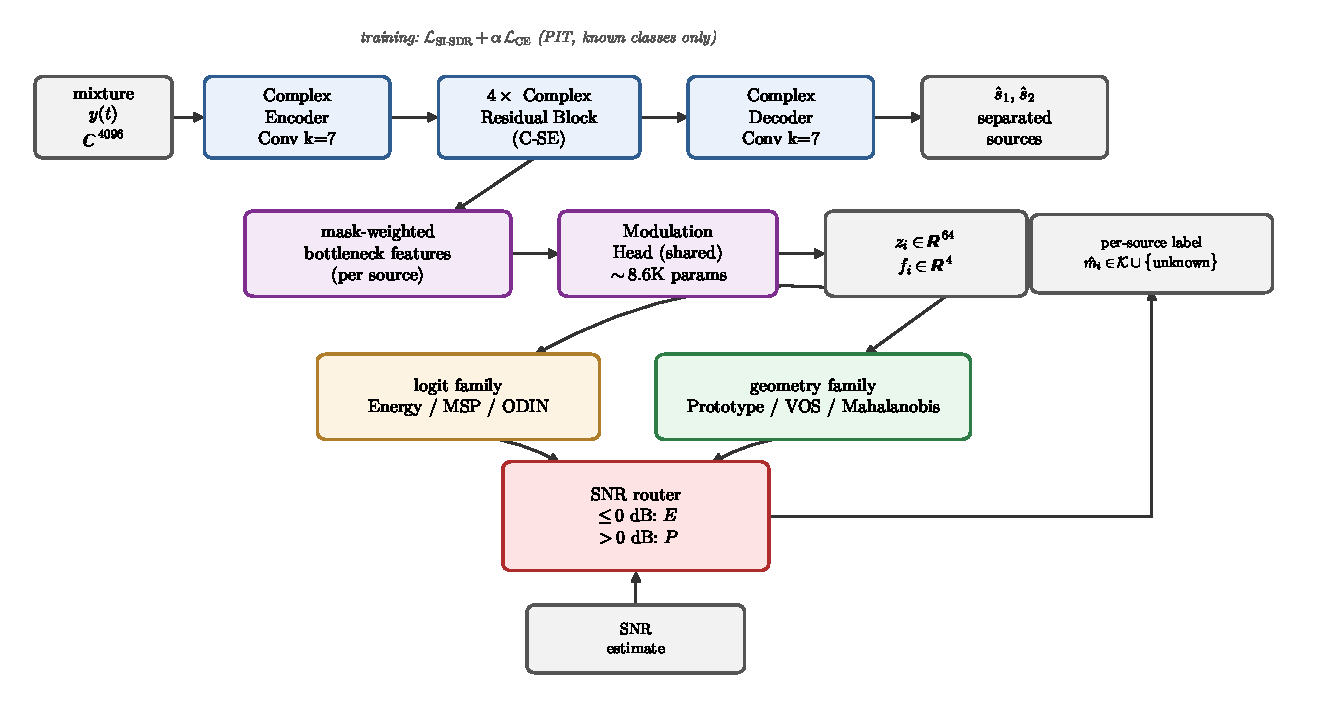
\includegraphics[width=\columnwidth]{figures/fig_architecture.pdf}
\caption{OpenSetCSE with SNR-routed OOD detection. Top: the C-SE
separation backbone. Bottom: the
shared per-source modulation head produces an embedding $z_i$ and
logits $f_i$; at inference, the SNR router selects the logit-family
score (Energy) at $\snr \leq \SI{0}{dB}$ and the geometry-family score
(Prototype) otherwise.}
\label{fig:arch}
\end{figure}

The separation backbone is a lightweight complex-valued CNN with
complex squeeze-and-excitation (C-SE) channel attention: a complex
encoder (ComplexConv1d + complex batch normalisation), a stack of four
complex residual blocks with C-SE, and a complex decoder producing two
separated waveforms $\hat{s}_1, \hat{s}_2 \in \mathbb{C}^{T}$. On top of the backbone, a
shared per-source \emph{modulation head} aggregates each output's
mask-weighted bottleneck features into a 64-dimensional embedding $z_i$
and $K=4$ logits $f_i$ (one per known modulation). The head adds
$\sim$8.6K parameters; the full model has $\sim$69K parameters.
Training is end-to-end with a permutation-invariant multi-task loss,
\begin{equation}
  \mathcal{L} = \mathcal{L}_{\text{SI-SDR}} + \alpha\,\mathcal{L}_{\text{CE}},
  \label{eq:loss}
\end{equation}
where $\mathcal{L}_{\text{SI-SDR}}$ is the scale-invariant
signal-to-distortion ratio (SI-SDR) loss under the PIT
convention~\cite{kolbaek2017pit,leroux2019sdr} and
$\mathcal{L}_{\text{CE}}$ is the cross-entropy of the per-source
modulation labels under the same permutation; we use $\alpha = 1$.
Only the four known modulations appear in training---no unknown-class
data, synthetic or real, is used at any stage.

\subsection{Per-source OOD scoring}
\label{sec:scorers}

Given per-source embeddings $z \in \mathbb{R}^{64}$ and logits
$f \in \mathbb{R}^{K}$, we evaluate six inference-time scorers (larger
= more OOD):
\begin{align}
  \text{Energy:}\quad
    E(f) &= -\log\textstyle\sum_k \exp f_k, \label{eq:energy}\\
  \text{Prototype:}\quad
    P(z) &= \min_k \| z - \mu_k \|_2, \label{eq:proto}\\
  \text{VOS:}\quad
    V(z) &= \min_j \| z - v_j \|_2, \label{eq:vos}\\
  \text{Mahalanobis:}\quad
    M(z) &= \min_k (z - \mu_k)^{\top} \Sigma^{-1} (z - \mu_k),
    \label{eq:maha}\\
  \text{MSP:}\quad
    S(f) &= -\max_k \mathrm{softmax}(f)_k, \label{eq:msp}\\
  \text{ODIN:}\quad
    O(x) &= -\max_k \mathrm{softmax}\!\big(f(\tilde{x}) / T\big)_k,
    \label{eq:odin}
\end{align}
with class prototypes $\mu_k$ (and the shared covariance $\Sigma$) fit
on the known pool, virtual outliers $v_j$ synthesised by extrapolation
from the class prototypes~\cite{du2022vos} (a training-free use of VOS:
no outlier-aware loss is applied), and ODIN~\cite{liang2018odin} using
temperature $T = 1000$ and a perturbation magnitude
$\varepsilon = 5\times10^{-3}$ extended to the complex mixture as
$\tilde{x} = x + \varepsilon\,(\mathrm{sign}\,\Re g + j\,\mathrm{sign}\,\Im g)$,
$g = \nabla_x \log\,\mathrm{softmax}(f/T)_{\hat{y}}$. Since no
unknown-class data is available at validation time by construction,
$\varepsilon$ is fixed a priori rather than tuned. The reference
statistics $(\mu_k, \Sigma, v_j)$ are computed on the known test pool;
a disjoint-reference-set check (Section~\ref{sec:expsetup}) shows this
choice is immaterial to every reported AUROC.

\subsection{SNR-routed ensemble}
\label{sec:routed}

The routing rule is fixed \emph{a priori} from the training/validation
SNR profile, not tuned on test data:
\begin{equation}
  \text{score}(z, f, \snr) =
  \begin{cases}
    E(f), & \snr \leq \SI{0}{dB},\\
    P(z), & \snr > \SI{0}{dB}.
  \end{cases}
  \label{eq:rule}
\end{equation}
Detection performance is reported as per-SNR-bin AUROC (known and
unknown pools at the same SNR), averaged across bins weighted by the
number of known$\,\times\,$unknown pairs---an SNR-conditioned detector
with per-bin operating points. In deployment the router uses an
\emph{estimated} SNR; sensitivity to estimation error is analysed in
Section~\ref{sec:robust}.

% ======================================================================
\section{Experiments}
\label{sec:exp}

\subsection{Setup}
\label{sec:expsetup}

\emph{Data.} All signals are synthetic complex baseband waveforms:
linear modulations (and OFDM-QPSK) with root-raised-cosine pulse
shaping, a three-tap multipath fading channel, and additive white
Gaussian noise~\cite{proakis2008digital}. Each mixture contains two
sources with carrier frequencies \SI{2000}{Hz} and \SI{2005}{Hz}
(each with an independent $\pm$\SI{5}{Hz} jitter) at
$T = 4096$ samples and a \SI{16}{kHz} sample rate. Training SNR is
uniform in $[-5, 20]$ dB; test SNR spans
$\{-10, -5, 0, 5, 10, 15, 20\}$ dB, i.e.\ including SNRs \emph{below}
the training range. Test sets are deterministic (fixed seed) with 200
mixtures per SNR for the kk/ku protocols and 100 for uu. No external
dataset is required; the generator is released with the code.

\emph{Training.} OpenSetCSE ($\sim$69K parameters), 100 epochs, batch
size 16, Adam at $10^{-3}$, loss of Eq.~\eqref{eq:loss} with
$\alpha = 1$. Five seeds (42--46).
\emph{Every} reported number is multi-seed: single-seed low-SNR results
proved unreliable twice in the course of this study, so no conclusion is
drawn from fewer than three seeds.

\emph{Reference pool.} The OOD reference statistics (prototypes
$\mu_k$, shared covariance $\Sigma$, virtual outliers $v_j$) are fit on
the known test pool. Re-fitting them on a disjoint held-out reference
set, generated under the same protocol with a fresh seed, changes every
AUROC reported below by less than 0.003; the choice of reference pool
is therefore immaterial to the conclusions.

\subsection{Closed-set sanity}
\label{sec:closed}

Table~\ref{tab:closed} shows that the backbone itself works: SI-SDR
turns positive at $\snr \geq \SI{10}{dB}$ and closed-set classification
accuracy is 0.41 (chance 0.25). The difficulty addressed in this paper
is genuinely in OOD detection, not separation.

\begin{table}[H]
\centering
\caption{Closed-set (kk) performance, 5-seed mean $\pm$ std.}
\label{tab:closed}
\begin{tabular}{lcc}
\toprule
Metric & Value \\
\midrule
Pooled SI-SDR (dB) & $-0.88 \pm 0.09$ \\
SI-SDR at \SI{10}{dB} (dB) & $+0.47 \pm 0.14$ \\
SI-SDR at \SI{20}{dB} (dB) & $+0.67 \pm 0.16$ \\
Classification accuracy & $0.407 \pm 0.030$ \\
\bottomrule
\end{tabular}
\end{table}

\subsection{The pooled-metric trap}
\label{sec:trap}

Pooled across SNR, \emph{all} scorers sit near chance
(Table~\ref{tab:trap}). The per-SNR breakdown
(Fig.~\ref{fig:persnr}) reveals why: Prototype/VOS reach
$0.84 \pm 0.02$ at \SI{10}{dB} but collapse below \SI{0}{dB}, while the
Energy score shows the \emph{opposite} profile, peaking at
$0.74 \pm 0.03$ at \SI{-5}{dB}. Pooled open-set metrics are misleading
for SC-BSS. (VOS and Prototype coincide to three decimals in every
aggregate we report---per-seed pooled AUROC differs by less than
0.002. Synthesised on a random shell around each class prototype, the
virtual outliers rarely reorder samples relative to the
nearest-prototype distance, so in this post-hoc setting the two scores
are effectively the same detector.)

\begin{table}[H]
\centering
\caption{Pooled OOD AUROC (all SNRs mixed), 5-seed mean $\pm$ std.
All scorers are near chance; the per-SNR structure is invisible here.}
\label{tab:trap}
\begin{tabular}{lc}
\toprule
Scorer & Pooled AUROC \\
\midrule
Energy      & $0.482 \pm 0.018$ \\
Prototype   & $0.509 \pm 0.013$ \\
VOS         & $0.509 \pm 0.013$ \\
Mahalanobis & $0.524 \pm 0.046$ \\
MSP         & $0.433 \pm 0.010$ \\
ODIN        & $0.486 \pm 0.016$ \\
\bottomrule
\end{tabular}
\end{table}

\begin{figure}[H]
\centering
\includegraphics[width=0.8\columnwidth]{figures/fig_per_snr_auroc.pdf}
\caption{Per-SNR OOD AUROC (5-seed mean). Energy and Prototype/VOS are
strongly complementary; the routed scorer follows the better branch.}
\label{fig:persnr}
\end{figure}

\subsection{SNR-routed ensemble}
\label{sec:main}

Routing lifts the weighted-average AUROC from 0.526 (the strongest
single scorer, Mahalanobis) to 0.625---a $+0.10$ gain obtained with
zero training cost (Table~\ref{tab:main}, Fig.~\ref{fig:overall}).
The gap to the post-hoc oracle (0.681) is small, indicating that the
two-branch rule captures most of the complementarity available from
all six scorers; the residual gap comes mainly from bins where a third
scorer (typically Mahalanobis at the extreme SNRs) wins without a
reliable a-priori rule to select it.

\begin{table}[H]
\centering
\caption{Main result: weighted-average per-SNR AUROC, 5-seed
mean $\pm$ std. Oracle = post-hoc best scorer per bin (upper bound).}
\label{tab:main}
\begin{tabular}{lc}
\toprule
Scorer & Weighted-avg AUROC \\
\midrule
Energy      & $0.487 \pm 0.032$ \\
Prototype   & $0.502 \pm 0.008$ \\
VOS         & $0.502 \pm 0.008$ \\
Mahalanobis & $0.526 \pm 0.043$ \\
MSP         & $0.435 \pm 0.012$ \\
ODIN        & $0.495 \pm 0.030$ \\
\midrule
\textbf{SNR-routed (ours)} & $\mathbf{0.625 \pm 0.031}$ \\
Oracle (post-hoc bound)    & $0.681 \pm 0.038$ \\
\bottomrule
\end{tabular}
\end{table}

\begin{figure}[!t]
\centering
\includegraphics[width=0.8\columnwidth]{figures/fig_overall_auroc.pdf}
\caption{Weighted-average AUROC: single scorers vs.\ SNR-routed ensemble
vs.\ oracle bound.}
\label{fig:overall}
\end{figure}

\subsection{Ablations}
\label{sec:ablations}

Two natural training-side interventions both fail, which is itself
informative:

\emph{Center loss} ($\lambda{=}0.1$, 5 seeds)~\cite{wen2016center}: no
aggregate gain (0.509 $\to$ 0.496 prototype AUROC); it weakens the
high-SNR prototype signal the router relies on (routed 0.568 vs.\
0.625). The known/unknown margin is not shaped by classification-side
losses.

\emph{Embedding dimension} (16/32/64/128, 3 seeds): closed-set and
routed AUROC are flat within seed noise (0.588--0.631, non-monotonic).
OOD performance is backbone-feature-limited, not capacity-limited.

\begin{table}[H]
\centering
\caption{Embedding-dimension ablation (3 seeds, mean $\pm$ std).}
\label{tab:embdim}
\begin{tabular}{lccc}
\toprule
Dim & Closed SI-SDR (dB) & Cls.\ acc & Routed AUROC \\
\midrule
16  & $-0.836 \pm 0.016$ & $0.422 \pm 0.007$ & $0.631 \pm 0.034$ \\
32  & $-0.864 \pm 0.004$ & $0.399 \pm 0.007$ & $0.588 \pm 0.010$ \\
64  & $-0.830 \pm 0.012$ & $0.424 \pm 0.003$ & $0.622 \pm 0.023$ \\
128 & $-0.891 \pm 0.057$ & $0.410 \pm 0.006$ & $0.618 \pm 0.021$ \\
\bottomrule
\end{tabular}
\end{table}

\subsection{Robustness to SNR-estimation error}
\label{sec:robust}

Even a poor ($\sigma = \SI{6}{dB}$) SNR estimator retains about half of
the routing gain and still outperforms the best single scorer
(Table~\ref{tab:robust}, Fig.~\ref{fig:robust}): mis-routing
only affects samples whose noisy estimate crosses the \SI{0}{dB}
decision boundary, i.e.\ the bins nearest to it, which is also where the
two scorers differ least. The demand placed on the SNR estimator is
therefore modest.

\begin{table}[H]
\centering
\caption{Routed AUROC when the routing decision uses a noisy SNR
estimate (50 Monte-Carlo trials per seed, 5 seeds).}
\label{tab:robust}
\begin{tabular}{lc}
\toprule
SNR-estimation noise $\sigma$ & Routed AUROC \\
\midrule
\SI{0}{dB} (ideal) & $0.625 \pm 0.031$ \\
\SI{1}{dB}         & $0.597 \pm 0.031$ \\
\SI{3}{dB}         & $0.593 \pm 0.030$ \\
\SI{6}{dB}         & $0.576 \pm 0.026$ \\
\bottomrule
\end{tabular}
\end{table}

\begin{figure}[!t]
\centering
\includegraphics[width=0.8\columnwidth]{figures/fig_snr_noise_robustness.pdf}
\caption{Graceful degradation under SNR-estimation error; the routed
scorer stays above the best single scorer (0.526) even at
$\sigma = \SI{6}{dB}$.}
\label{fig:robust}
\end{figure}

\subsection{Robustness to carrier-frequency separation}
\label{sec:freqgap}

The baseline model is trained at a \SI{5}{Hz} carrier gap between the
two sources. Evaluating it at gaps from \SI{10}{Hz} to \SI{500}{Hz}
(Table~\ref{tab:freqgap}) leaves the routed gain essentially unchanged
(0.615--0.633, within seed noise), showing that the SNR-routing
conclusion is not an artefact of the training carrier separation. Single
scorers remain near chance at every gap, so the pooled-metric trap is
equally present at all separations.

\begin{table}[H]
\centering
\caption{Weighted-avg per-SNR AUROC vs.\ carrier-frequency separation
(5 seeds; model trained at \SI{5}{Hz} gap).}
\label{tab:freqgap}
\begin{tabular}{lccc}
\toprule
Carrier gap & Energy & Prototype & Routed \\
\midrule
\SI{5}{Hz} (train) & 0.487 & 0.502 & $0.625 \pm 0.031$ \\
\SI{10}{Hz}        & 0.488 & 0.500 & $0.625 \pm 0.034$ \\
\SI{50}{Hz}        & 0.486 & 0.509 & $0.631 \pm 0.035$ \\
\SI{100}{Hz}       & 0.488 & 0.497 & $0.633 \pm 0.035$ \\
\SI{500}{Hz}       & 0.533 & 0.529 & $0.615 \pm 0.043$ \\
\bottomrule
\end{tabular}
\end{table}

\subsection{Qualitative analysis}
\label{sec:qual}

Fig.~\ref{fig:pca} projects the per-source embeddings of one seed to
their first two principal components. At $\snr \leq \SI{0}{dB}$ the
embeddings form a single overlapping cloud in which known and unknown
modulations are largely indistinguishable, apart from a partially
separated BPSK lobe. At $\snr \geq \SI{10}{dB}$ the known classes
contract and concentrate, and the unknown modulations (crosses) drift
away from the known mass. The 2-D projection only hints at this
separation, which the per-SNR AUROC of the distance-based scorers in
Fig.~\ref{fig:persnr} quantifies ($0.84$ at \SI{10}{dB}); it is the
geometric picture behind their high-SNR effectiveness and their
low-SNR collapse.

\begin{figure}[!t]
\centering
\includegraphics[width=0.85\columnwidth]{figures/fig_embedding_pca.pdf}
\caption{PCA of per-source embeddings (seed 42) at low vs.\ high SNR.
At high SNR the known classes concentrate and the unknown modulations
(crosses) drift away from the known mass; at low SNR known and unknown
overlap in a single cloud. The 2-D projection understates the
separation quantified in Fig.~\ref{fig:persnr}.}
\label{fig:pca}
\end{figure}

% ======================================================================
\section{Discussion}
\label{sec:disc}

\emph{Why does the Energy score invert at high SNR?} The energy family
(Energy, MSP, ODIN) reads out the logit distribution of a classifier
trained only on known classes. At low SNR, unknown-modulation signals
produce near-uniform logits---their features do not match any learned
template---while known signals still elicit a peaked response, so the
scores separate (0.74 AUROC at \SI{-5}{dB}). At high SNR the classifier
becomes over-confident on \emph{every} input, known or not: the logit
spread collapses, all samples look alike to a confidence-based scorer,
and the ranking inverts (Energy falls to 0.22 at \SI{10}{dB}).

\emph{Why does the geometry family invert the other way?} Prototype,
VOS and Mahalanobis scores measure distances in embedding space, and
distances are only meaningful once the embedding itself carries class
structure. The PCA view (Fig.~\ref{fig:pca}) hints at that structure
emerging only at moderate-to-high SNR; below \SI{0}{dB} the embeddings
of all signals collapse to noise-like clouds in which known and unknown
are indistinguishable (Prototype $\approx 0.35$--$0.42$). Once the
backbone has effectively de-noised its inputs, unknown modulations land
measurably far from the known prototypes (0.84 at \SI{10}{dB}).

\emph{The two ablations support this picture.} If the SNR dependence
were a matter of head capacity or of classification-side shaping, a
wider embedding or center loss would improve the routed AUROC; neither
helps---the embedding dimension is flat within seed noise, and center
loss actively \emph{degrades} routing (0.568 vs.\ 0.625) by weakening
the high-SNR prototype signal the router relies on. The SNR dependence
is a property of the \emph{backbone features}, not of the readout.

\emph{Generality.} Routing requires only a scalar operating-condition
estimate and a per-scorer competence profile---both available a priori
from validation data. The same recipe applies wherever OOD detectability
is condition-dependent (other channel impairments, other tasks), and it
composes with any post-hoc scorer: the gains reported here are obtained
with off-the-shelf scorers and zero retraining. The per-source head
costs $\sim$8.6K parameters and routing is a table lookup, so the
deployed overhead over the closed-set separator is negligible.

% ======================================================================
\section{Limitations and Future Work}
\label{sec:limit}

Routing uses an (estimated) SNR; a learned soft router may do better.
Symbols are assumed aligned; data are synthetic; scenarios are
two-source. Training-side fixes that directly optimise the known/unknown
margin (e.g.\ VOS with synthetic outliers in the loss) remain unexplored,
as does mixture-level (rather than per-source) OOD detection.

% ======================================================================
\section{Conclusion}
\label{sec:concl}

We have presented the first open-set formulation of single-channel blind
source separation for co-frequency communication signals: joint
separation with per-source rejection of unseen modulations. On this
benchmark, standard pooled OOD metrics are actively misleading---all six
scorers we evaluated sit near chance when averaged over SNR---because
per-source detectability is SNR-dependent: logit-based scores separate
known from unknown only at low SNR, geometry-based scores only at high
SNR. Exploiting this complementarity with a training-free SNR-routed
ensemble lifts the weighted-average AUROC from 0.526 to 0.625 (5 seeds),
within 0.06 of the post-hoc oracle, robustly to SNR-estimation error and
to a $100\times$ change in carrier separation. Multi-seed ablations show
the effect lives in the backbone features, not in the head. We hope the
benchmark and the pooled-metric trap it exposes will push both the
SC-BSS and the OOD communities toward condition-aware evaluation.

% ======================================================================
\section*{CRediT authorship contribution statement}
\textbf{Bin Nong:} Conceptualization, Methodology, Software, Validation,
Formal analysis, Investigation, Data curation, Writing -- original
draft, Visualization.
\textbf{Weihong Fu:} Supervision, Project administration, Writing --
review \& editing.
\textbf{Zhuoyun Jiang:} Resources, Validation, Writing -- review \&
editing.

\section*{Declaration of competing interest}
The authors declare that they have no known competing financial
interests or personal relationships that could have appeared to
influence the work reported in this paper.

\section*{Data availability}
Code and synthetic data generators are available at
\url{https://github.com/BinNong/single_channel_source_seperation/tree/main/paper3_open_set}.
No external datasets are required.

\section*{Funding}
This research did not receive any specific grant from funding agencies
in the public, commercial, or not-for-profit sectors.

\section*{Declaration of generative AI and AI-assisted technologies in the writing process}
During the preparation of this work the authors used Claude Code
(Anthropic) in order to assist with drafting, editing, and polishing the
manuscript text. After using this tool, the authors reviewed and edited
the content as needed and take full responsibility for the content of
the publication.

% ======================================================================
% Bibliography ordered by first citation (elsarticle numbered style).
\begin{thebibliography}{30}\footnotesize

\bibitem{hou2022single}
X.~Hou and Y.~Gao,
``Single-channel blind separation of co-frequency signals based on
convolutional network,''
\emph{Digital Signal Processing}, vol.~129, p.~103654, 2022,
doi:~\url{https://doi.org/10.1016/j.dsp.2022.103654}.

\bibitem{guo2024single}
P.~Guo, M.~Yu, L.~Shen, Z.~Lin, K.~An, and J.~Wang,
``Single-channel blind source separation in wireless communications: a
complex-domain deep learning approach,''
\emph{IEEE Wireless Commun. Lett.}, vol.~13, no.~6, pp.~1645--1649,
2024, doi:~\url{https://doi.org/10.1109/LWC.2024.3384813}.

\bibitem{bendale2016openmax}
A.~Bendale and T.~E. Boult,
``Towards open set deep networks,''
in \emph{Proc. CVPR}, 2016, pp.~1563--1572,
doi:~\url{https://doi.org/10.1109/CVPR.2016.173}.

\bibitem{hendrycks2017msp}
D.~Hendrycks and K.~Gimpel,
``A baseline for detecting misclassified and out-of-distribution
examples in neural networks,''
in \emph{Proc. ICLR}, 2017.

\bibitem{liang2018odin}
S.~Liang, Y.~Li, and R.~Srikant,
``Enhancing the reliability of out-of-distribution image detection in
neural networks,''
in \emph{Proc. ICLR}, 2018.

\bibitem{liu2020energy}
W.~Liu, X.~Wang, J.~D. Owens, and Y.~Li,
``Energy-based out-of-distribution detection,''
in \emph{Proc. NeurIPS}, 2020.

\bibitem{hyvarinen2000ica}
A.~Hyv{\"a}rinen and E.~Oja,
``Independent component analysis: algorithms and applications,''
\emph{Neural Netw.}, vol.~13, no.~4--5, pp.~411--430, 2000,
doi:~\url{https://doi.org/10.1016/S0893-6080(00)00026-5}.

\bibitem{chen2019deep}
C.~Chen, Z.~Lu, Z.~Guo, F.~Yang, and L.~Ding,
``Deep learning based single-channel blind separation of co-frequency
modulated signals,''
in \emph{Proc. ChinaCom}, 2019, pp.~607--618,
doi:~\url{https://doi.org/10.1007/978-3-030-41114-5_45}.

\bibitem{ma2023novel}
H.~Ma, X.~Zheng, L.~Yu, et~al.,
``A novel end-to-end deep separation network based on attention
mechanism for single channel blind separation in wireless
communication,''
\emph{IET Signal Process.}, vol.~17, no.~2, p.~e12173, 2023,
doi:~\url{https://doi.org/10.1049/sil2.12173}.

\bibitem{luo2023single}
W.~Luo, R.~Yang, H.~Jin, et~al.,
``Single channel blind source separation of complex signals based on
spatial-temporal fusion deep learning,''
\emph{IET Radar, Sonar Navig.}, vol.~17, no.~2, pp.~200--211, 2023,
doi:~\url{https://doi.org/10.1049/rsn2.12333}.

\bibitem{s4unet2026}
S.~Gao, W.~Guo, H.~Shi, and R.~Peng,
``S4-UNET: a long-sequence modeling blind source separation method for
single-channel co-channel overlapped communication signals,''
\emph{J. Electron. Inf. Technol.}, vol.~48, no.~6, pp.~2384--2395,
2026, doi:~\url{https://doi.org/10.11999/JEIT251144}.

\bibitem{deng2024co}
W.~Deng, X.~Wang, and Z.~Huang,
``Co-channel multiuser modulation classification using data-driven blind
signal separation,''
\emph{IEEE Internet Things J.}, vol.~11, no.~8, pp.~14829--14843, 2024,
doi:~\url{https://doi.org/10.1109/JIOT.2023.3345023}.

\bibitem{trabelsi2018complex}
C.~Trabelsi, O.~Bilaniuk, Y.~Zhang, D.~Serdyuk, S.~Subramanian,
J.~F. Santos, S.~Mehri, N.~Rostamzadeh, Y.~Bengio, and C.~J. Pal,
``Deep complex networks,''
in \emph{Proc. ICLR}, 2018.

\bibitem{lee2022complex}
C.~Lee, H.~Hasegawa, and S.~Gao,
``Complex-valued neural networks: a comprehensive survey,''
\emph{IEEE/CAA J. Autom. Sinica}, vol.~9, no.~8, pp.~1406--1426, 2022,
doi:~\url{https://doi.org/10.1109/JAS.2022.105743}.

\bibitem{hu2018senet}
J.~Hu, L.~Shen, and G.~Sun,
``Squeeze-and-excitation networks,''
in \emph{Proc. CVPR}, 2018, pp.~7132--7141,
doi:~\url{https://doi.org/10.1109/CVPR.2018.00745}.

\bibitem{scheirer2013open}
W.~J. Scheirer, A.~de~Rezende~Rocha, A.~Sapkota, and T.~E. Boult,
``Toward open set recognition,''
\emph{IEEE Trans. Pattern Anal. Mach. Intell.}, vol.~35, no.~7,
pp.~1757--1772, 2013, doi:~\url{https://doi.org/10.1109/TPAMI.2012.256}.

\bibitem{lee2018mahalanobis}
K.~Lee, K.~Lee, H.~Lee, and J.~Shin,
``A simple unified framework for detecting out-of-distribution samples
and adversarial attacks,''
in \emph{Proc. NeurIPS}, 2018.

\bibitem{du2022vos}
X.~Du, Z.~Wang, M.~Cai, and Y.~Li,
``VOS: Learning what you don't know by virtual outlier synthesis,''
in \emph{Proc. ICLR}, 2022.

\bibitem{dhamija2018oscr}
A.~Dhamija, M.~G{\"u}nther, and T.~Boult,
``Reducing network agnostophobia,''
in \emph{Proc. NeurIPS}, 2018.

\bibitem{wen2016center}
Y.~Wen, K.~Zhang, Z.~Li, and Y.~Qiao,
``A discriminative feature learning approach for deep face
recognition,''
in \emph{Proc. ECCV}, 2016, pp.~499--515,
doi:~\url{https://doi.org/10.1007/978-3-319-46478-7_31}.

\bibitem{proakis2008digital}
J.~G.~Proakis and M.~Salehi,
\emph{Digital Communications}, 5th~ed., McGraw-Hill, 2008.

\bibitem{oshea2017intro}
T.~O'Shea and J.~Hoydis,
``An introduction to deep learning for the physical layer,''
\emph{IEEE Trans. Cogn. Commun. Netw.}, vol.~3, no.~4, pp.~563--575,
2017, doi:~\url{https://doi.org/10.1109/TCCN.2017.2758370}.

\bibitem{kolbaek2017pit}
M.~Kolb{\ae}k, D.~Yu, Z.-H. Tan, and J.~Jensen,
``Multitalker speech separation with utterance-level permutation
invariant training of deep recurrent neural networks,''
\emph{IEEE/ACM Trans. Audio, Speech, Lang. Process.}, vol.~25, no.~10,
pp.~1901--1913, 2017,
doi:~\url{https://doi.org/10.1109/TASLP.2017.2726762}.

\bibitem{leroux2019sdr}
J.~Le~Roux, S.~Wisdom, H.~Erdogan, and J.~R.~Hershey,
``SDR---half-baked or well done?,''
in \emph{Proc. ICASSP}, 2019, pp.~626--630,
doi:~\url{https://doi.org/10.1109/ICASSP.2019.8683855}.

\end{thebibliography}

\end{document}
